%%%% Proceedings format for most of ACM conferences (with the exceptions listed below) and all ICPS volumes.
\documentclass[sigconf, nonacm=true, natbib=true]{acmart}
%%%% Proceedings format for SIGPLAN conferences 
% \documentclass[sigplan, anonymous, review]{acmart}
% \usepackage[sorting=none]{biblatex}
\usepackage{booktabs} % For formal tables
\usepackage{amsmath}
%\usepackage{algorithm}
\usepackage{algpseudocode}
%\usepackage{graphicx}
\usepackage[vlined, ruled, boxed]{algorithm2e}
%\usepackage{enumitem}
\usepackage[]{algorithm2e}


\setcopyright{none}
% % DOI
% \acmDOI{10.475/123_4}
% % ISBN
% \acmISBN{123-4567-24-567/08/06}
% %Conference
% \acmConference[WOODSTOCK'97]{ACM Woodstock conference}{July 1997}{El Paso, Texas USA}
% \acmYear{1997}
% \copyrightyear{2016}
\acmDOI{}
\acmYear{}
\acmISBN{}
\acmConference{}
\acmArticle{}
\acmArticleSeq{0}
\acmPrice{}


\begin{document}
\title{CSE6140 Fall 2018 Project \\Traveling Salesperson Problem (TSP)}
\subtitle{Implementation and Evaluation of
Four Algorithms}
%\subtitlenote{The full version of the author's guide is available as \texttt{acmart.pdf} document}


\author{Dongmin Han}
%\authornote{Dr.~Trovato insisted his name be first.}
\orcid{1234-5678-9012}
\affiliation{%
  \institution{Mechanical Engineering}
}
\email{hdmhust@gmail.com}

\author{Shan Xiong}
\affiliation{%
  \institution{Mechanical Engineering}
}
\email{sxiong33@gatech.edu}

\author{Chong Ye}
\affiliation{%
  \institution{Mechanical Engineering}
}
\email{chongtt.ye@gmail.com}

\author{Yuanlai Zhou}
\affiliation{%
  \institution{Computational Science \& Engineering}
}
\email{yuanlai.zhou@gmail.com}
% % The default list of authors is too long for headers.
% \renewcommand{\shortauthors}{B. Trovato et al.}

\begin{abstract}
In this paper, we adopted four different algorithms to find optimal or "good" solution to this problem, including branch and bound, construction heuristics with approximation guarantees (MST-approx), local search with simulated annealing (SA) and generic algorithm (GA). We have also evaluated their theoretical and experimental complexities on real world instances. \\
\hfill\\
To get optimal solutions, we used penalty-based selection strategy in the Branch-and-Bound algorithm to obtain good quality of lower bound. Over half of all the given cases have been solved within 1.5 hours. Approximation algorithm in all the given cases takes less than 0.1 sec per case and can achieve solution qualities better than 40\%. Local search algorithms are generally fast and can produce satisfactory results with carefully optimized parameters. All the given cases can be solved with qualities better than 15\% within 2 minutes in our experiments with GA and SA algorithms.  
\\
% For the checkpoint of this project, we implemented two approaches: branch and bound (BnB), and Local search (LS) with generic algorithm. The results are shown in the follow sections. \textbf{Also, we'd like to participate the project competition (Team 31)}.

%\footnote{This is an abstract footnote}
\end{abstract}

% The code below should be generated by the tool at
% http://dl.acm.org/ccs.cfm
% Please copy and paste the code instead of the example below.
%
% \begin{CCSXML}
% <ccs2012>
%  <concept>
%   <concept_id>10010520.10010553.10010562</concept_id>
%   <concept_desc>Computer systems organization~Embedded systems</concept_desc>
%   <concept_significance>500</concept_significance>
%  </concept>
%  <concept>
%   <concept_id>10010520.10010575.10010755</concept_id>
%   <concept_desc>Computer systems organization~Redundancy</concept_desc>
%   <concept_significance>300</concept_significance>
%  </concept>
%  <concept>
%   <concept_id>10010520.10010553.10010554</concept_id>
%   <concept_desc>Computer systems organization~Robotics</concept_desc>
%   <concept_significance>100</concept_significance>
%  </concept>
%  <concept>
%   <concept_id>10003033.10003083.10003095</concept_id>
%   <concept_desc>Networks~Network reliability</concept_desc>
%   <concept_significance>100</concept_significance>
%  </concept>
% </ccs2012>
% \end{CCSXML}

% \ccsdesc[500]{Computer systems organization~Embedded systems}
% \ccsdesc[300]{Computer systems organization~Redundancy}
% \ccsdesc{Computer systems organization~Robotics}
% \ccsdesc[100]{Networks~Network reliability}

\keywords{Traveling salesperson problem, Branch and bound, Approximation, Heuristics, Local search, Generic algorithm, Simulated annealing}
\maketitle

\section{Introduction}
The traveling Salesperson Problem (TSP) is a well-known NP-complete problem with numerous applications, such as transportation, planning, and logistics. In this study, we implemented four algorithms to solve the TSP with instances from real world database. These algorithms include branch-and-bound (BnB), construction heuristics (approximation) and two versions of local search (LS). All four algorithms are successfully implemented and evaluated with a systematic empirical analysis. 

\section{Problem Definition}
Given the $x-y$ coordinates of $N$ points in the plane (i.e., vertices) and a cost function $c(u,v)$ defined for every pair of points (i.e., edge), find the shortest simple cycle that visits all $N$ points.\\
\\
The cost function $c(u,v)$ is defined as either the Euclidean or Geographic distance between points $u$ and $v$. Specifically, for the \textbf{EUC\_2D} format, we have $x-y$ coordinates of $u$ and $v$, which are $(u_x, u_y)$ and $(v_x, v_y)$, respectively. Then we can easily calculated the cost function (pairwise distance) by the following equation:
\begin{equation}
  c(u,v)=\sqrt[]{(u_x-v_x)^2 + (u_y-v_y)^2}
\end{equation}
The results will be rounded to the nearest integer for the following computation.\\
\\
For \textbf{GEO} format, the $x-y$ coordinates (latitude and longitude) will first be converted to radii. Then we take the floor of $x$ and $y$ coordinates. The distance $d_{ij}$ between points $i$ and $j$ can be calculated by the following steps:
\begin{itemize}
\item Step 1. Converting to radius
\begin{align*}
\pi &= 3.141592;\\
deg &= \lfloor x_i\rfloor;\\
min &= \pi (deg+5/3 min)/180
\end{align*} 
\item Step 2. Calculating the geographical distance
\begin{align*}
q_1 &= \cos(longitude[i]-longitude[j]);\\
q_2 &= \cos(latitude[i]-latitude[j]);\\
q_3 &= \cos(latitude[i]+latitude[j]);\\
d_{ij}&=\lfloor R \times \arccos[0.5q_2(1.0+q_1) - 0.5q_3(1.0-q_1)]+1.0\rfloor \\
(R &= 6378.388 km) 
\end{align*}
\end{itemize}
The proposed solution will provide a valid simple cycle that visits all the $N$ points, together with its total length. An optimal solution will give the cycle with shortest total length.



\section{Related Work}
\subsection{Exact Algorithm: Branch-and-Bound}
In 1963, John D. C. Little et al \cite{Little1963} proposed a Branch-and-Bound algorithm for solving the traveling salesman problem. The set of all tours (feasible solutions) is broken up into increasingly small subsets by a procedure called branching. For each subset a lower bound on the length of the tours therein is calculated. Eventually, a subset is found that contains a single tour whose length is less than or equal to some lower bound for every tour. The motivation of the branching and the calculation of the lower bounds are based on ideas frequently used in solving assignment problems. Computationally, the algorithm extends the size of problem that can reasonably be solved without using methods special to the particular problem. This is also one of the algorithms that we adopted in this study.\\
\\
In 2014, M. Battarra \textit{et al} proposed three mathematical formulations as exact algorithms for the TSP \cite{Battarra2014}. The first algorithm is a branch-and-cut approach and is based on a compact formulation in which two sets of two-index binary variables and a polynomial number of constraints are employed. When strengthened with subtour elimination constraints and trivial constrains, this method is not empirically dominated by the best formulation proposed by Rakke et al \cite{glomvik2012}. The second algorithm is also a branch-and-cut, but the underlying formulation considers three index variables. It is proven to dominate the first method, both theoretically and empirically. The last method is a branch-cut-and-price and is based on a Dantzig-Wolfe decomposition of the second formulation. Columns are generated by dynamically introducing $ng$-paths to the formulation. This method is capable of solving to optimality all the benchmark instances from the literature.\\
\\
Exact approaches to solving the TSP are successfully
adopted only for relatively small problem sizes, although they can guarantee optimality based on different techniques. They usually use algorithms that generate both a lower and an upper bound on the true minimum value of the problem instance. If the upper and lower bound coincide, a proof of optimality is achieved. 
Due to the nature of TSP, most common solutions to
the problem were found to run feasibly only for a graph
with small number of nodes. Not much research was
encountered in the survey over problem space analysis of
the Traveling Salesman problem.

\subsection{Construction Heuristics with Approximation Guarantees}
Golden and Stewart proposed the CCAO algorithm in 1985. This heuristic was designed for symmetrical Euclidean TSPs. It exploits a well-known property of such problems, namely that in any optimal solution, vertices located on the convex hull of all vertices are visited in the order in which they
appear on the convex hull boundary (Flood, 1956). One major drawback of the CCAO algorithm is that its insertion phase is myopic in the following sense: since insertions are executed sequentially without much concern for global optimality, they may result in a succession of bad decisions that the post-optimization phase will be unable to undo.\\
\\
In 1992, Gendreau, Hertz and Laporte proposed the GENIUS algorithm to improve this type of algorithm. GENIUS executes each insertion more carefully, by performing a limited number of local transformation of the tour, simultaneously with the insertion itself. It consists of two parts: a generalized insertion phase, followed by a post-optimization phase that successively removes vertices from the tour and reinserts them, using the generalized insertion rule.\\
\\
This algorithm has been extensively tested on randomly generated problems and on problems taken from the literature; all these problems were symmetrical and Euclidean. Tests revealed that GENIUS produces in shorter computing times
better solutions than CCAO, superior to all tour construction heuristics developed in this section. This algorithm also appears to compare favourably to tabu search and simulated annealing, although the number of comparisons was more limited in the case of these two methods.

\subsection{Local Search}
In 2008, S. Basu et al \cite{Basu2008}  presented
a survey of Tabu search approach for solving the TSP. As per the literature survey, the tabu search is said to be most widely used Meta heuristic procedures to solve combinatorial optimization problems. It is an improvement heuristic based on local search. It starts with an initial solution to the problem, (a tour in case of the TSP), calls it a current solution, and searches for the best solution in a suitably defined neighborhood of the solution. It then designates the best solution in the neighborhood as the current solution and starts the search process again. Tabu search terminates when
certain terminating conditions, either involving execution
time or maximum iteration count conditions, or solution
quality objectives, or both, have been met.\\
\\
% In 2011, A Philip cite{philip2011} a Genetic Algorithm (GA) for solving the TSP. Genetic Algorithm is a very good local search algorithm and is employed to solve the TSP by generating a preset number of random tours and then improving the population until a stop condition is satisfied and the best path is returned as the solution. Analysis of the algorithmic parameters (Population, Mutation Rate and Cut Length) was done so as to know how to tune the algorithm for various problem instances. The program produced good results for various problem sizes but run time increases with increasing number of cities. To get good solutions a tradeoff must be made between runtime and the solution quality.
In 2011, Z. Hlaing \cite{chi2011} presented an approach for solving the TSP based on improved ant colony algorithm. The main contribution of this work is a study of the avoidance of stagnation behavior and premature convergence by using distribution strategy of initial ants and dynamic heuristic parameter updating based on entropy. Then a mergence of local search solution is provided. The experimental results
and performance comparison showed that the proposed system reaches the better search performance over ACO algorithms do.\\
\\
In 2012, V. Dwivedi et al \cite{Dwivedi2012} proposed a new crossover operator for a genetic algorithm to solve the TSP. The crossover is the important stage in the genetic algorithm. A new crossover method called Sequential Constructive Crossover (SCX) operator is adopted. The SCX uses best edges of the parent’s structure and produces the new offspring. It is compared against other existing crossover operators and it is proved that SCX results in a high quality solutions. This paper also includes a comparative study on Greedy Approach, Dynamic Programming and Genetic Algorithm for solving TSP. 


\section{Algorithms}
\subsection{Branch-and-Bound}
\subsubsection{Introduction of BnB}
\hfill\\
A branch-and-bound (BnB) algorithm consists of a systematic enumeration of all candidate solutions, where large subsets of fruitless candidates are discarded by using upper and lower estimated bounds of the quantity being optimized. The BnB strategy divides a problem into a number of sub-problems. It is a system for solving a sequence of subproblems, each of which may have multiple possible solutions and where the solution chosen for one sub-problem may affect the possible solutions of later sub-problems.\\
\\
Suppose it is required to minimize an objective function. Suppose that we have a method for getting a lower bound on the cost of any solutions among those in the set of solutions represented by some subset. If the best solution found so far costs less than the lower bound for this subset, we need not explore this subset at all.\\
\\
Let $S$ be some subset of solutions. $LB(S) = $ a lower bound on the cost of any solutions $\in S$. Let $C = $ cost of the best solution found so far. Then if $C \leq LB(S)$, there is no need to explore $S$ since it does not contain any better solutions. If $C > LB(S)$, then we need to continue exploring $S$.

\subsubsection{Outline of BnB}
\hfill\\
We adopted an algorithm proposed by John D. C. Little et al \cite{Little1963} in 1963. We will use the following example\cite{Bnb-Poth2013} to show the outline of this algorithm. Consider a TSP within five cities (vertices), which form an undirected, connected graph. The following Cost Matrix shows the distance between the five cities. 
$$
\text{Cost Matrix} =  
\bordermatrix{
          & 1 & 2 & 3 & 4 & 5     \cr
    1     & - & 10 & 8 & 9 & 7    \cr
    2     & 10 & - & 10 & 5 & 6   \cr
   	3 	  & 8 & 10 & - & 8 & 9    \cr
    4     & 9 & 5 & 8 & - & 6   \cr   
    5     & 7 & 6 & 9 & 6 & -   \cr
            }
$$
As discussed in the Algorithm class, we first reduce the matrix using the minimum number in each row and each column. The sum of the row and column minimum will give us the lower bound, which is $7+5+8+5+6=31$ (row), $31+1=32$ (row + column). After this reduction, we obtain the reduced matrix as follows:
% Reduced Matrix = 
% \bordermatrix{
%           & 1 & 2 & 3 & 4 & 5    \cr
%     1     & - & 3 & 0 & 2 & 0    \cr
%     2     & 5 & - & 4 & 0 & 1    \cr
%     3 	& 0 & 2 & - & 0 & 1    \cr
%     4     & 4 & 0 & 2 & - & 1    \cr   
%     5     & 1 & 0 & 2 & 0 & -    \cr
%             }
$$
\text{Reduced Matrix} =  
\bordermatrix{
          & 1 & 2 & 3 & 4 & 5     \cr
    1     & - & 3 & 0^{(2)} & 2 & 0^{(1)}    \cr
    2     & 5 & - & 4 & 0^{(1)} & 1   \cr
   	3 	  & 0^{(1)} & 2 & - & 0^{(0)} & 1    \cr
    4     & 4 & 0^{(1)} & 2 & - & 1   \cr   
    5     & 1 & 0^{(0)} & 2 & 0^{(0)} & -   \cr
            }
$$
Note that in the reduced matrix, for each $Zero$, a penalty number is labeled in the bracket. This penalty number is calculated by adding up the lowest numbers (other than this $Zero$) from the same row and column as this particular $Zero$. This means if we don't make the assignment in this $Zero$, we will incur an additional cost equals to this penalty. Consider $X_{13}$ since it has the highest penalty. If we don't have the path from 1 to 3, i.e., $X_{13}=0$, then we will have an additional cost of 2 and the lower bound becomes $32+2=34$. \\
\\
On the other hand, if we have the path from 1 to 3, i.e., $X_{13}=1$, we will eliminate the respective row and column to explore the next path within the remaining cities (vertices). The remaining matrix is as follows:\\
$$
\text{Remaining Matrix} =  
\bordermatrix{
          & 1 & 2 & 4 & 5   \cr
    2     & 5 & - & 0 & 1   \cr
   	3 	  & - & 2 & 0 & 1   \cr
    4     & 4 & 0 & - & 1   \cr   
    5     & 1 & 0 & 0 & -   \cr
            }
$$
Do the reduction for column 1 and column 5, and update the current lower bound to $32+1+1=34$. Calculate the penalties for all the $Zero's$ in the newly reduced matrix, select the one with highest penalty 3, which is $X_{51}$. If $X_{51}=0$, lower bound will be updated to $LB = 34 +3 =37$. If $X_{51}=1$, eliminate row 5 and column 1 with the $LB = 34$ unchanged. The remaining matrix becomes:
$$
\text{Remaining Matrix} =    
\bordermatrix{
           & 2 & 4 & 5   \cr
    2      & - & 0^{(0)} & 0^{(0)}   \cr
   	3 	   & 2 & 0^{(2)} & -   \cr
    4      & 0^{(2)} & - & 0^{(0)}   \cr   
            }
$$
No more reduction is needed and the penalties are labeled in the matrix. Consider $X_{34}$ since it has the highest penalty. If $X_{34}=0$, $LB = 34+2=36$. If $X_{34}=1$, we obtain the following matrix with $LB = 34$ unchanged:
$$
\text{Remaining Matrix} =    
\bordermatrix{
           & 2 & 5   \cr
    2      & -  & 0   \cr
    4      & 0  & -   \cr   }
$$
Here we have $Zero's$ in each row and column, and the bound will remain the same $LB= 34+0=34$. We now obtain a feasible solution by assigning $X_{25}=1$ and $X_{42}=1$. The solution is $X_{13}+X_{34}+X_{42}+X_{25}+X_{51}=34$, which is corresponding to the path 1-3-4-2-5-1.
The following figure shows the decision tree of this example:\\ 
\begin{figure}[h]
    \centering
    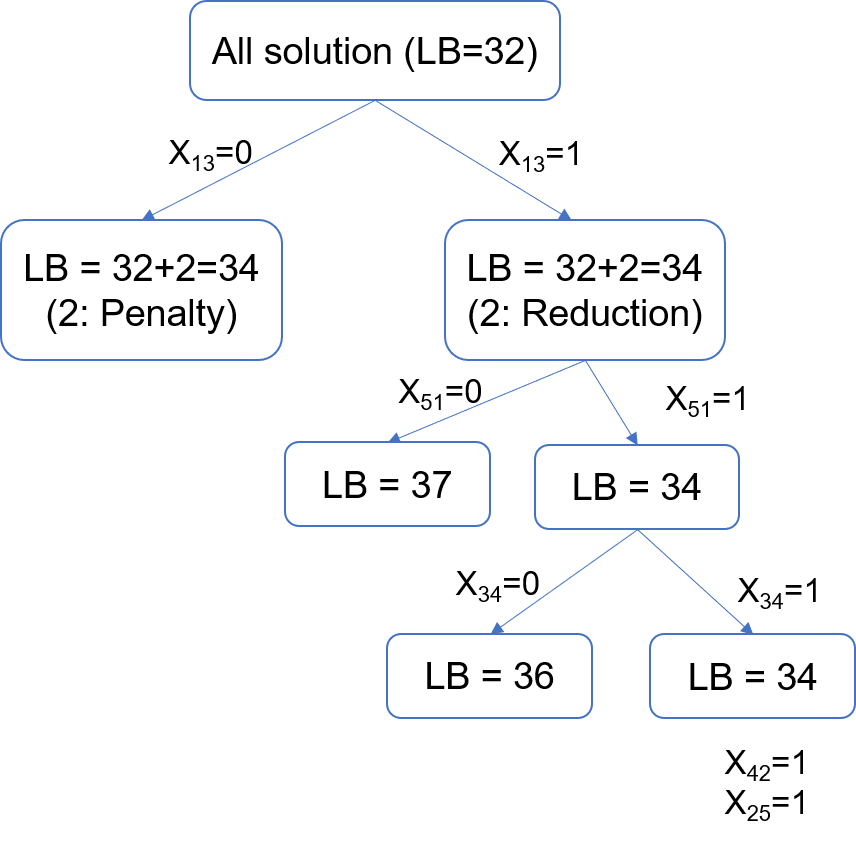
\includegraphics[width=0.35\textwidth]{Bnb-example}
    \caption{Decision Tree for an Example of BnB Algorithm}
    \label{fig:Bnb}
\end{figure}
\\
The above proposed solution for the example is following the right branch in the figure \ref{fig:Bnb} and it gives us an upper bound ($UB = 34$) for feasible solutions. Since all the left branches in each step have a larger than the proposed solution ($LB \geq UB$), the proposed solution is optimal. In other cases, if there exits a certain branch with $LB < UB$, then the algorithm should go back to this level and explore this branch to see if it gives a better solution. In the end, this BnB algorithm will provide the optimal solution given long enough time. 
\subsubsection{Complexity Analysis of BnB}
\hfill\\
The worst case time complexity of Branch-and-Bound algorithm remains the same as that of the Brute Force, which is $O(2^n)$, because in worst case, we may never get a chance to prune a node. Nevertheless, in practice, it may perform very well depending on the different instance of the TSP.\\
\\
The worst case space complexity is $O(2^n\cdot n^2)$ since we need a $n\times n$ matrix in the beginning, two $(n-1)\times (n-1)$ matrices in the second level, ..., and $2^{n-2}$ ($2\times 2$) matrices in the lowest level, because in the worst case, we may never get a chance to prune a node and need to consider all the branches expanded in each step. Nevertheless, in practice, it may perform very well when most of the branches can be pruned when the first solution is obtained, which only requires $O(n^3)$ in terms of space complexity.
\subsubsection{Pseudo-code of BnB}
\hfill\\
The pseudo-code for BnB algorithm is shown in \textbf{Algorithm 1\&2}.
\begin{algorithm}
 \KwData{$n$ nodes with $x-y$ coordinates $(x_i, j_i)$}
 \KwResult{a path that visits all the $n$ nodes, total length}
 Global variable: cost[N][N] \Comment{cost matrix}\\
 \textbf{function} CheckBounds(str,end,cost[n][n]) \\
 $pencost[0]=t$\\
 \For{$i$ $\leftarrow$ $0, n-1$}
 {
 \For{$j$ $\leftarrow$ $0, n-1$}
 {$reduced[i][j]=cost[i][j]$}
 }
 \For{$j$ $\leftarrow$ $0, n-1$}
 {
 $reduced[str][j]]=\infty$
 }
 \For{$i$ $\leftarrow$ $0, n-1$}
 {
 $reduced[i][end]]=\infty$
 }
 $reduced[end][str]=\infty$\\
 $RowReduct(reduced)$\\
 $ColReduct(reduced)$
 $pencost[end] = pencost[str] + row +col+cost[str][end]$
\textbf{return} $pencost[end]$\\

 \textbf{function} RowMin(cost[n][n], i)\\
 $min=cost[i][0]$\\
 \For{$j$ $\leftarrow$ $0, n-1$}
 {
 \If{$cost[i][j]<min$}
 {$min = cost[i][j]$}
 }
 \textbf{return} min\\
 
 \textbf{function} ColMin(cost[n][n], i)\\
 $min=cost[0][j]$\\
 \For{$i$ $\leftarrow$ $0, n-1$}
 {
 \If{$cost[i][j]<min$}
 {$min = cost[i][j]$}
 }
 \textbf{return} min\\
 
 \textbf{function} RowReduct(cost[n][n])\\
 $row=0$\\
 \For{$i$ $\leftarrow$ $0, n-1$}
 {
 $rmin=rowmin(cost,i)$\\
   \If{$cmin \neq \infty$}
   {$row = row + rmin$}
 \For{$j$ $\leftarrow$ $0, n-1$}
  {
  \If{$cost[i][j] \neq \infty$}
  {$cost[i][j]=cost[i][j]-rmin$}
  }
 }
 
 \textbf{function} ColReduct(cost[n][n])\\
 $col=0$\\
 \For{$j$ $\leftarrow$ $0, n-1$}
 {
 $cmin=columnmin(cost,j)$\\
   \If{$cmin \neq \infty$}
   {$col = col + cmin$}
 \For{$i$ $\leftarrow$ $0, n-1$}
  {
  \If{$cost[i][j] \neq \infty$}
  {$cost[i][j]=cost[i][j]-cmin$}
  }
 }

 
 
\caption{BnB algorithm}
\end{algorithm}

%====================BnB con't=====================%
\begin{algorithm}
 \textbf{function} Main()\\
 \For{$i$ $\leftarrow$ $0, n-1$}
 {
 $select[i]=0$
 }
 $rowreduct(cost)$\\
 $colreduct(cost)$\\
 $t = row + col$\\
  \While{$allvisited(select) \neq 1$}
  {
  \For{$i$ $\leftarrow$ $1, n-1$}
  	{\If{$select[i]=0$}
     	{
         $edgecost[i]=checkbounds(k,i,cost)$
         }
     }
    $min=\infty$\\
   \For{$i$ $\leftarrow$ $1, n-1$}
   {
     \If{$select[i]=0$}
     {
         \If{$edgecost[i]<min$}
         {
         $min=edgecost[i]$\\
         $k=i$
         }
     }
   }
  $select[k]=1$\\
  \For{$p$ $\leftarrow$ $1, n-1$}
  	{$cost[j][p]=\infty$
    }
  \For{$p$ $\leftarrow$ $1, n-1$}
  	{$cost[p][k]=\infty$}
  $cost[k][j]=\infty$\\
  rowreduct(cost)\\
  colreduct(cost)\\
  }
 
\caption{BnB algorithm (con't)}
\end{algorithm}



%=============================================%

\subsection{Construction Heuristics with Approximation Guarantees}
\subsubsection{Introduction of Approximation Algorithm}
\hfill\\
There are several approaches for dealing with NP-complete problems (TSP here). We have worked on exact solution via BnB approach as shown in Section \textbf{4.1}, although it may take super long time in some cases. Sometimes, we need a quick, yet good enough solution, this is where the approximation algorithm fits in. Approximation algorithms run in polynomial time and always produce a solution close to the optimal. We called an algorithm an $\alpha$-approximation algorithm if it runs in polynomial time, and always outputs a solution that is at most $\alpha \cdot$OPT for a minimization problem (or at least 1/$\alpha \cdot$OPT for a maximization problem), where OPT denote the optimal value. Note that we must have $\alpha \geq$ 1 and it does not have to be a constant. Here we will discuss approximation algorithms for the Traveling Salesman Problem.\\

In the Traveling Salesman Problem, we are given a complete graph G with nonnegative edge costs, and the goal is to find a minimum-cost cycle that visits every vertex exactly once. The key to designing approximation algorithm is to obtain a bound on the optimal value OPT. In the case of TSP, the minimum spanning tree (MST) gives a lower bound on OPT. This is the algorithm that we have discussed in the class, and we will solve the TSP with this MST-Approx algorithm.\\


\subsubsection{Outline of MST-Approximation Algorithm}
\hfill\\
MST-approximation gives us a simple 2-approximation algorithm for metric TSP. The algorithm is as follows:
\begin{enumerate}
\item  Take the minimum-weight spanning tree (MST) of the TSP graph.The MST can be computed in polynomial time using Kruskal's or Prim's algorithm\cite{Tardos}.
\item Do a depth-first search (DFS) of the MST, hitting every edge exactly twice. This "pseudo-tour" PT has the cost of $2 \times$ MST $\leq 2 \times $ OPT. Write down each vertex as it is visited.
\item Rewrite the list of vertices, writing each vertex only the first time it appears in PT. Thus PT will be converted to the tour as required by TSP.

\end{enumerate}


\subsubsection{Complexity Analysis of MST-Approximation Algorithm}
\hfill\\
The time complexity of MST algorithm is $O(n^2)$. The DFS step takes $O(n+m)$. Therefore, the total time complexity of MST-Approximation is $O(n^2)$. It takes $O(n)$ to store the sequence of nodes visited and $O(n^2)$ to store the distance matrix between each two cities in the beginning. We can see that this approximation algorithm is very efficient with a guarantee of solution quality within $2\times$OPT. It is very useful if we need a rough estimation of the solution quickly, but it may not give us very good quality compared to other optimization algorithms given longer computing time.\\



\subsection{Local Search 1: Genetic Algorithm}
\subsubsection{Basic introduction}
\hfill\\
Genetic algorithms are inspired by Darwin's theory about evolution. Solution to a problem solved by genetic algorithms is evolved.\\
\\Algorithm is started with a set of solutions (represented by chromosomes) called population. Solutions from one population are taken and used to form a new population. This is motivated by a hope, that the new population will be better than the old one. Solutions which are selected to form new solutions (offspring) are selected according to their fitness - the more suitable they are the more chances they have to reproduce\cite{Cezary1991}. This is repeated until some condition (for example number of populations or improvement of the best solution) is satisfied.

\subsubsection{Outline of Genetic Algorithm}
\hfill\\
1. (Start) Generate random population of n chromosomes (suitable solutions for the problem)\\
2. (Fitness) Evaluate the fitness f(x) of each chromosome x in the population\\
3. (New population) Create a new population by repeating following steps until the new population is complete\\
\indent 3.1 (Selection) Select two parent chromosomes from a population according to their fitness (the better fitness, the bigger chance to be selected)\\
\indent 3.2 (Crossover) With a crossover probability cross over the parents to form a new offspring (children). If no crossover was performed, offspring is an exact copy of parents.\\
\indent 3.3 (Mutation) With a mutation probability mutate new offspring at each position in chromosome\\
\indent 3.4 (Accepting) Place new offspring in a new population\\
4. (Replace) Use new generated population for a further run of algorithm\\
5. (Test) If the end condition is satisfied, stop, and return the best\\ solution in current population\cite{Intro2GA}\\
6. (Loop) Go to step 2

\subsubsection{Example}
\hfill\\
\begin{figure}
    \centering
    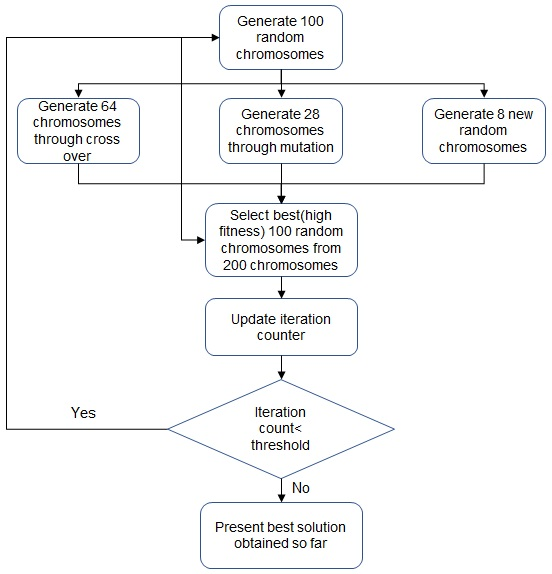
\includegraphics[width=0.48\textwidth]{flowchart}
    \caption{Flow chart of Genetic Algorithm}
    \label{fig: GA}
\end{figure}
A specific example of Genetic Algorithm is as follows\cite{TutorialGA}.\\
\textbf{1. Generate chromosomes}\\
We assume that there are 7 cities, we can generate an array of size 6 like below.\\
\begin{center}
\begin{tabular}{ |c|c|c|c|c|c|c| }
\hline
 Random number&0.23&0.65&0.49&0.58&0.75&0.34 \\
 \hline
 Sequence & 2 & 3& 4& 5& 6& 7 \\ 
 \hline
\end{tabular}
\end{center}
Then we sort the array based on the first row. After this, the sequence in second row give us a chromosome, that is, $1->2->7->4->5->3->6->1$.\\
We can further repeat this process to generate the required number of chromosomes.\\
\hfill\\
\textbf{2. Cross over}\\
We use two parent chromosomes to form a new offspring.\\
\begin{center}
\begin{tabular}{|c|c|c|c|c|c|c|c|}
\hline
Parent1 & 1& 3& 4& 2& \emph{5}& \emph{7}& \emph{6} \\
\hline
Parent2 & 1& \emph{7}& \emph{5}& 2& 3& 4& \emph{6} \\
\hline
Offspring & 1& 2& 3& 4& \emph{5}& \emph{7}&\emph{6}\\
\hline
\end{tabular}
\end{center}
As the table shows, we use $5,7,6$ of Parent1 for cross over. We further remove $5,7,6$ from Parent2.Finally, we get $1,2,3,4$ from Parent2 and $5,7,6$ from Parent1 to form a new offspring.\\
\hfill\\
\textbf{3. Mutation}\\
We use one parent to generate offspring through mutaion.\\
\begin{center}
\begin{tabular}{ |c|c|c|c|c|c|c|c| } 
 \hline
 Parent1 & 1 & 3& \emph{4}& \emph{2}& \emph{5}& 7& 6 \\
 \hline
 Offspring & 1 & 3& \emph{5}& \emph{2}& \emph{4}& 7& 6 \\ 
 \hline
\end{tabular}
\end{center}
As the table shows, we can mutate the Parent1 by changing the position of $4,5$ to form a new offspring.\\
\hfill\\
\textbf{4.Flow chart}\\
The Figure \ref{fig: GA} shows us the process of Genetic Algorithm based on above comments. Here we assume that population size is 100.
% \begin{figure}
%     \centering
%     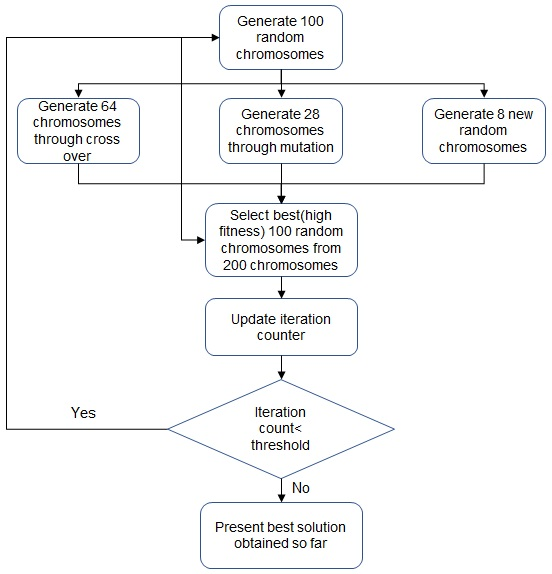
\includegraphics[width=0.48\textwidth]{flowchart}
%     \caption{Flow chart of Genetic Algorithm}
%     \label{fig: GA}
% \end{figure}

\subsubsection{Complexity Analysis of GA}
\hfill\\
We assume that g: number of generations, n: population size and m:  size of the individuals, Genetic Algorithms complexity is $O(g(nm + nm + n))$. So, the time complexity is $O(gnm)$.\\
Since the population size is n and individuals size is m, we have n arrays and each has size m. So, the space complexity is $O(nm)$.

%==========================================================%

\subsection{Local Search 2: Simulated Annealing} 
\subsubsection{Introduction}
\hfill\\
Simulated annealing algorithm (SA) is a stochastic local search technique inspired by the physical process of annealing.Annealing is a controlled heating and cooling process of metals to improve its strength. It allows worsening steps for the overall optimal solution. Analogous to the metal annealing process, when the temperature is high, atoms are moving around easily. And when it is cooling down, atoms moving slows down and tend to find configuration with lower internal energy. Similarly, higher temperature means more probability to accept worsening steps and lower temperature means shrinking the probability of accepting worse neighboring solution, thus focusing on improving moves.\\
\hfill\\
The probability of accepting the neighboring solution over the current solution could be determined by Metropolis condition shown below: \\
\[P(s', s)=\Big\{
\begin{tabular}{cc}
1 & if \(f(s') > f(s)\)\\
\(exp \left\{
\frac{f(s')-f(s)}{T}
\right\}
\) & otherwise
\end{tabular}
\]
As the probability condition shown above, it is obvious that when the neighboring solution is superior than the current solution evaluate by evaluation function, the neighboring solution is accepted. However, if the neighboring solution is worse, whether to choose the neighboring solution over the current solution depends on the probability which is related to the temperature. As the temperature is decreasing, the probability of accepting neighboring solution is decreasing as well. 
In the SA algorithm, it is also important to choose how to update the temperature and determine stopping criterion. Sometimes, we may also need to restart the algorithm and move back to a previous solution which is better than the current solution. 


\subsubsection{Outline of Simulated Annealing Algorithm}
\hfill\\
The baseline implementation of SA for TSP is showing as follows:
\begin{enumerate}
\item Start with a random initial solution \(S_0\) and set the initial temperature \(T_0\), calculate the total lengthe of the initial sulution \(f(s_0)\). Initialize \(i=0\).
\item \(T = T_i\). Use two-exchange neighborhood method to form neighboring solution \(S'\) and calculate the total length of the neighboring solution. Take T, \(S_i\) and \(S'\) to Metropolis criterion and return the solution \(S\). The current iteration \(i=i+1\) and the solution to the current state is \(S_i=S\).
\begin{enumerate}
\item Calculate the total lengths of old solution \(f(s_i)\) and new neighboring solution \(f(s')\) respectively and their difference as \(\Delta f=f(s')-f(s_i) \).
\item If \(\Delta f>0\), then return the new neighboring solution \(S'\). Ohterwise, take the new neighboring solution according to probability P.
\end{enumerate}
\item Reduce the temperature based on some criterion and ensure \(T_i<T_{i-1}\). Evaluate the current solution, it stop criterion is satisfied, go to the next step Otherwise, return to step (2).
\item Return the current solution and terminate the algorithm.
\end{enumerate}


\subsubsection{Complexity Analysis of Simulated Annealing Algorithm}
\hfill\\
Time and space complexity of implementing simulated annuealing algorithm to solve for TSP is \(O(n)\). 
The outer loop of temperature iteration takes \(O(a)\) time steps. At a specific temperature, the inner loop takes \(O(b)\) time steps. Thus, the time complexity of the SA algorithm for TSP is \(O(n)\).

\subsubsection{Pseudo-code of Simulated Annealing}
\hfill\\
The pseudo-code for simulated annealing algorithm is shown in \textbf{Algorithm 3}.
\begin{algorithm}
 \KwResult{solution, state}
 \textbf{function} Simulated Annealing(problem, schedule) \\
 $ current \leftarrow Make-Node(Initial-State[Problem]) $\\
 \For{$t$ $\leftarrow$ 1 to infinity (iters,time cutoff)}
 {
 $ T \leftarrow schedule[t] $\\
 \If{$T=0$}
 {\textbf{return} greedy from current\\}
 $ next \leftarrow Random-successor(current) $\\
 $ \Delta E \leftarrow f-Value[next]-f-value[current] $\\
 \If{$ \Delta E > 0$}
 {$ current \leftarrow next $\\}
 $ else $\\
 $ current \leftarrow next with probability $
 }
 
\caption{Simulated Annealing algorithm}
\end{algorithm}

%=============================================================%

\section{Empirical Evaluation}
\subsection{Comprehensive Table}
All of the code is implemented by desktop with CPU: Intel i7-6700 8 core and RAM: 16G.
\subsubsection{Branch-and-Bound Algorithm}
\hfill\\
The current results of Branch-and-Bound algorithms are shown in the table shown below. We tried to get as good results as possible with long period of runtime (up to 16 hours). The optimal solution is obtained from the NOES solver as stated in Acknowledgement.\\
\begin{center}
\begin{tabular}{ |c|c|c|c|c| }
\hline
City         & Opt. Sol. & Result  & Elap.Time & Sol.Qual. \\
\hline
Atlanta      & 2003763   & 2003763 & 0.09      & 0.00      \\
Berlin       & 7542      & 7542    & 4834      & 0.00      \\
Boston       & 893536    & 893536  & 6.7       & 0.00      \\
Champaign    & 52643     & 52643   & 2400      & 0.00      \\
Cincinnati   & 277952    & 277952  & 0.006     & 0.00      \\
Denver       & 100431    & 123156  & 1944      & 3.64      \\
NYC          & 1555060   & 1611626 & 29668     & 3.64      \\
Philadelphia & 1395981   & 1395981 & 55489     & 0.00      \\
Roanoke      & 655454    & 832259  & 600       & 26.97     \\
SanFrancisco & 810196    & 944471  & 18093     & 16.57     \\
Toronto      & 1176151   & 1593793 & 40172     & 35.51     \\
UKansasState & 62962     & 62962   & 0.019     & 0.00      \\
ulysses16    & 6859      & 6859    & 0.01      & 0.00      \\
Umissouri    & 132709    & 145512  & 600       & 9.65      \\ 
\hline

%  \hline
%  City & Elap.Time (s) & Sol.Qual.\\
%  \hline
%  Atlanta & 6.70 & 893536 \\ 
%  \hline
%  Berlin & 0.09 & 2003763 \\
%  \hline
%  Boston & 600 & 53047 \\ 
%  \hline
%  Champaign & 0.01 & 277952 \\ 
%  \hline
%  Cincinnati & 0.02 & 62962 \\
%  \hline
%  Denver & 0.01 & 6756 \\
%  \hline
%  NYC & 600 & 7832 \\
%  \hline
%  Philadelphia & 600 & 1481183 \\
%  \hline
%  Roanoke & 600 & 123828 \\ 
%  \hline
%  SanFrancisco & 600 & 1632222 \\ 
%  \hline
%  Toronto & 600 & 832259 \\ 
%  \hline
%  UKansasState & 600 & 145512 \\
%  \hline
%  ulysses16 & 600 & 1595032 \\ 
%  \hline
%  Umissouri & 600 & 946164 \\ 
%  \hline
\end{tabular}
\end{center}

\subsubsection{Construction Heuristics with Approximation Guarantees}
\hfill\\
\begin{center}
\begin{tabular}{ |c|c|c|c| } 
\hline
City         & Result  & Elap.Time & Sol.Qual. \\
\hline
Atlanta      & 2270785 & 0         & 13.33     \\
Berlin       & 9550    & 0.02      & 26.62     \\
Boston       & 1028494 & 0.02      & 15.10     \\
Champaign    & 62395   & 0.02      & 18.52     \\
Cincinnati   & 297490  & 0         & 7.03      \\
Denver       & 133065  & 0.02      & 32.49     \\
NYC          & 2003747 & 0.02      & 28.85     \\
Philadelphia & 1626820 & 0.02      & 16.54     \\
Roanoke      & 808235  & 0.09      & 23.31     \\
SanFrancisco & 1060717 & 0.03      & 30.92     \\
Toronto      & 1618300 & 0.05      & 37.59     \\
UKansasState & 65561   & 0.02      & 4.13      \\
ulysses16    & 7788    & 0.02      & 13.54     \\
Umissouri    & 165116  & 0.02      & 24.42     \\
\hline
\end{tabular}
\end{center}


\subsubsection{Local Search 1: Genetic Algorithm}
\hfill\\
The current results of Genetic Algorithm and Simulated Annealing are shown in the table below. The maximum run time is cut off to 2 minutes. The results shown in the table below are the best results achieved in 2 minutes with average value after running 10 times.\\
\begin{center}
\begin{tabular}{ |c|c|c|c| } 
 \hline
 City        & Result  & Elap.Time & Sol.Qual. \\
 \hline
Atlanta      & 2003763 & 8.23      & 0.00      \\
Berlin       & 8020    & 35.12     & 6.34      \\
Boston       & 912650  & 61.27     & 2.14      \\
Champaign    & 54143   & 52.7      & 2.85      \\
Cincinnati   & 277952  & 0.07      & 0.00      \\
Denver       & 109210  & 108.43    & 8.74      \\
NYC          & 1623724 & 65.06     & 4.42      \\
Philadelphia & 1398906 & 13.8      & 0.21      \\
Roanoke      & 720217  & 117.4     & 9.88     \\
SanFrancisco & 876175  & 95.23     & 8.14      \\
Toronto      & 1306955 & 114.72    & 11.12     \\
UKansasState & 62962   & 0.04      & 0.00      \\
ulysses16    & 6859    & 2.06      & 0.00      \\
Umissouri    & 141931  & 104.18    & 6.95     \\
\hline
\end{tabular}
\end{center}

\subsubsection{Local Search 2: Simulated Annealing}
\hfill\\
\begin{center}
\begin{tabular}{ |c|c|c|c| } 
 \hline
 City         & Result  & Elap.Time & Sol.Qual. \\
 \hline
Atlanta      & 2102361 & 4.13      & 4.92      \\
Berlin       & 8340    & 34.61     & 10.58     \\
Boston       & 941078  & 18.52     & 5.32      \\
Champaign    & 56416   & 33.68     & 7.17      \\
Cincinnati   & 277952  & 0.17      & 0.00      \\
Denver       & 108190  & 77.16     & 7.73      \\
NYC          & 1690590 & 54.71     & 8.72      \\
Philadelphia & 1459913 & 12.34     & 4.58      \\
Roanoke      & 753432  & 117.87    & 14.95     \\
SanFrancisco & 906497  & 110.28    & 11.89     \\
Toronto      & 1313056 & 118.6     & 11.64     \\
UKansasState & 62980   & 0.13      & 0.03      \\
ulysses16    & 6997    & 2.16      & 2.01      \\
Umissouri    & 144095  & 112.44    & 8.58     \\
\hline
\end{tabular}
\end{center}

\subsection{Evaluation Plots for LS Algorithms}
In this section, we will use multiple plots to evaluate the performance of two Local Search (LS) algorithms, namely, Generic Algorithm (GA) and Simulated Annealing (SA) algorithm. We selected two cities, Berlin and Champaign, as the samples to analyze. They are selected because, 1. we are confident about the exact optimal solutions for these two cities, therefore we can obtain accurate errors/quality ranges for the evaluation, and 2. the input sizes of these two cities are large enough and will take a while (>100s) to obtain solutions with good qualities (within $15\% \cdot$ quality), which will make more sense in terms of performance evaluations and comparisons.\\
\hfill\\
For each algorithm and each city, 100 independent experiments with random seeds are performed. The evaluation plots are shown as follows.

\subsubsection{Qualified Runtime for Various Solution Qualities (QRTDs)}
\hfill\\
The qualified runtime distributions for various solution qualities for two cities using Generic Algorithm (GA) are shown in Figure \ref{fig: GA-QRTD}. The plot using Simulated Algorithm (SA) is shown in Figure \ref{fig: SA-QRTD}.\\
\hfill\\
From QRTD plots, we can see that for higher solution tolerance (lower quality bar such as 30\%, 35\%), the curve shifts to the left, meaning we can obtain good enough solutions (high probability) within shorter time. This is reasonable and therefore the algorithms are feasible. We can also see that SA can achieve similar qualities within shorter times, since it can quickly converge to a solution with the controlled cooling process.  

% \begin{figure}[h]
%     \centering
%     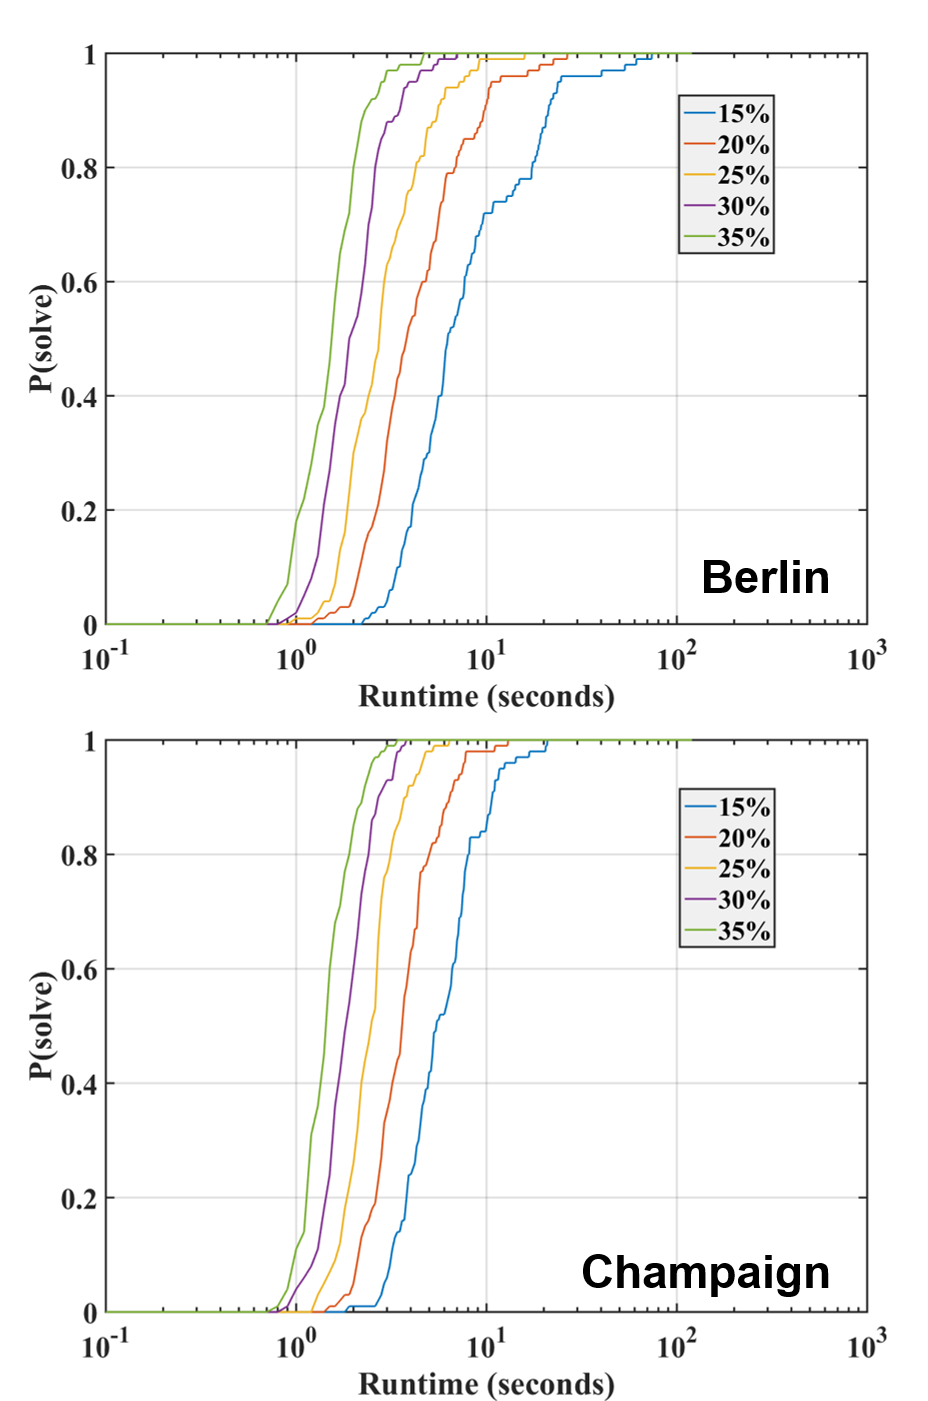
\includegraphics[width=0.35\textwidth]{F1-GA-QRTD}
%     \caption{QRTD plot using GA for Berlin and Champaign}
%     \label{fig: GA-QRTD}
% \end{figure}


% \begin{figure}[h]
%     \centering
%     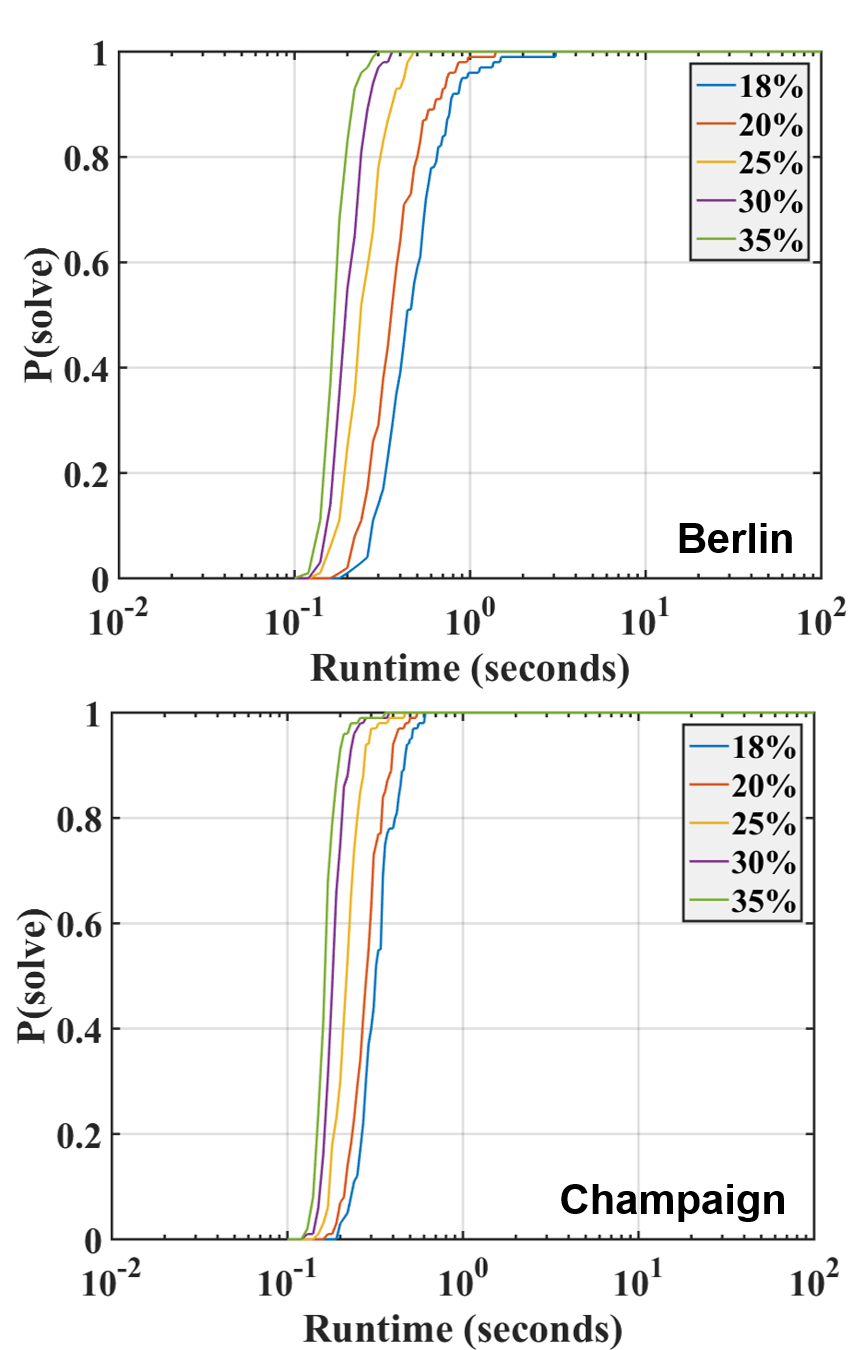
\includegraphics[width=0.35\textwidth]{F2-SA-QRTD}
%     \caption{QRTD plot using SA for Berlin and Champaign}
%     \label{fig: SA-QRTD}
% \end{figure}



\begin{figure}
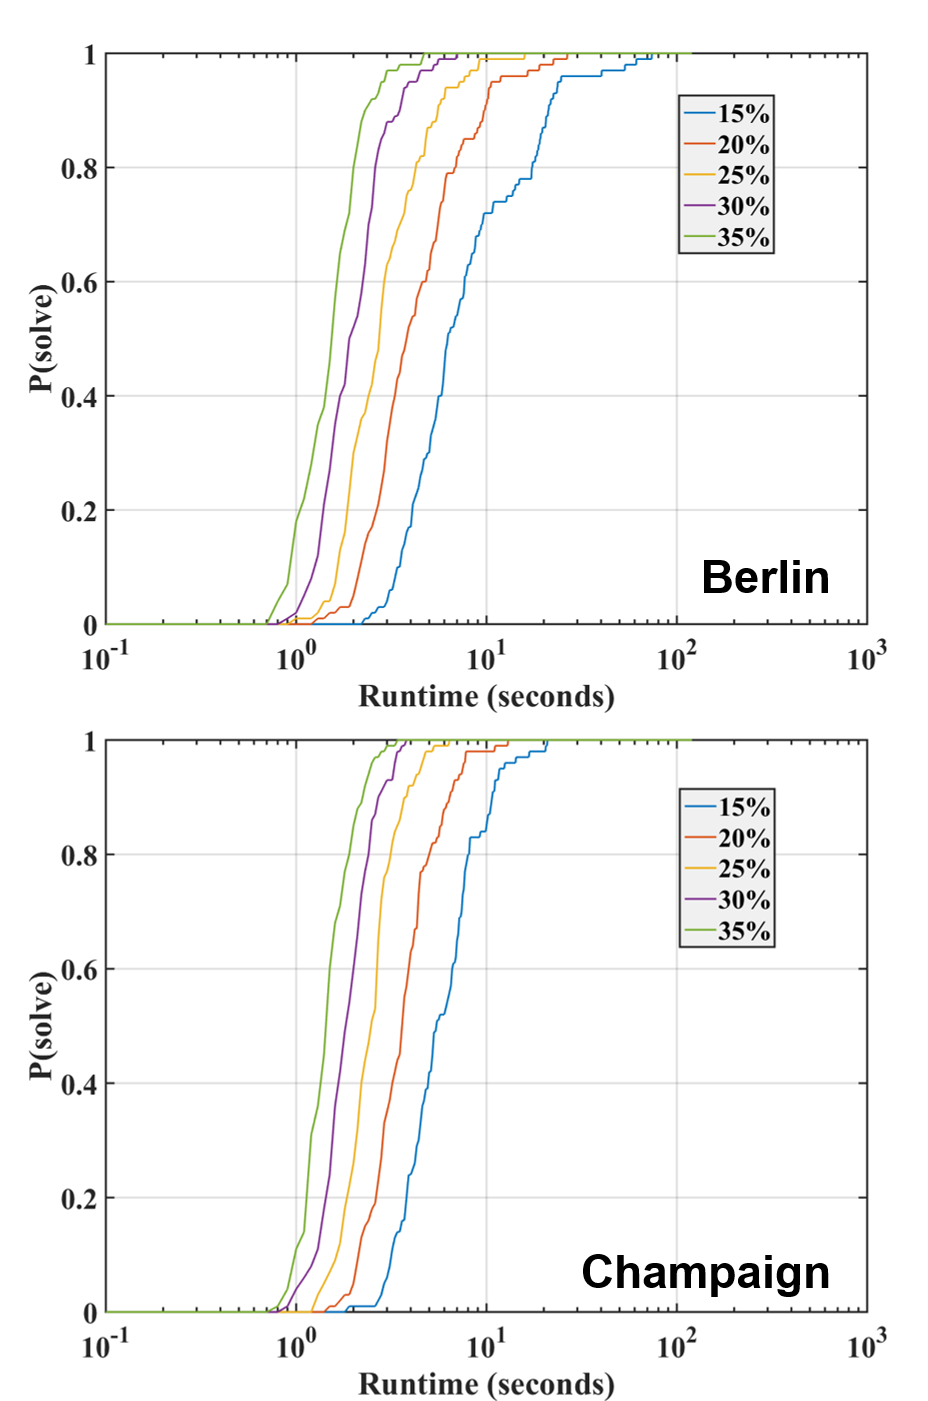
\includegraphics[width=2.5in]{F1-GA-QRTD}
\caption{QRTD plot using GA for Berlin and Champaign}
\label{fig: GA-QRTD}
\end{figure}


\begin{figure}
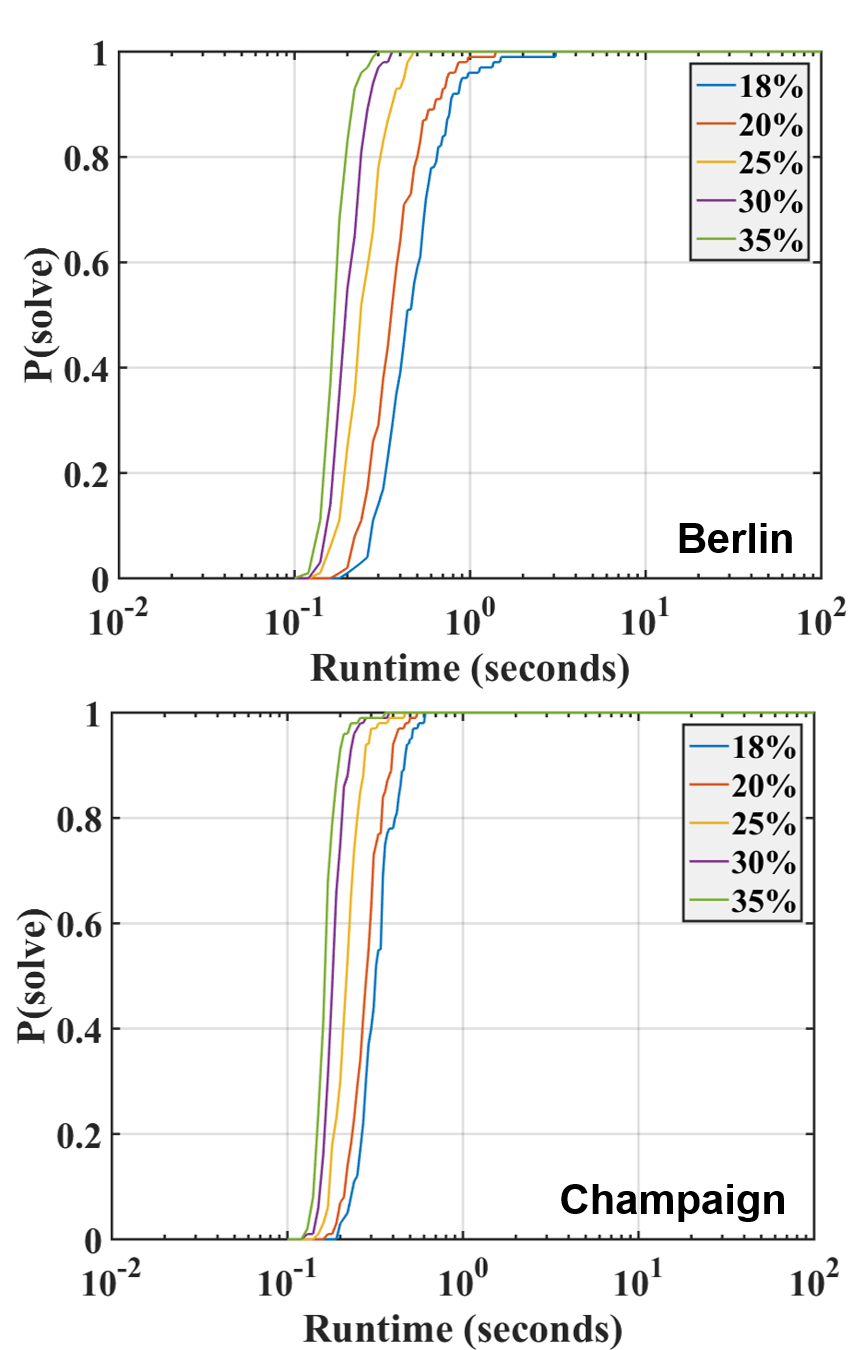
\includegraphics[width=2.5in]{F2-SA-QRTD}
\caption{QRTD plot using SA for Berlin and Champaign}
\label{fig: SA-QRTD}
\end{figure}


\subsubsection{Solution Quality Distributions (SQDs)}
\hfill\\
The SQD plots for two cities using Generic Algorithm (GA) are shown in Figure \ref{fig: GA-SQD}. The plot using Simulated Algorithm (SA) is shown in Figure \ref{fig: SA-SQD}.\\
\hfill\\
From SQD plots, we can see that for longer cutoff times, the curve shifts to the left, meaning we can obtain better enough solutions more easily. This is reasonable and therefore the algorithms are feasible. 
% \begin{figure}[h]
%     \centering
%     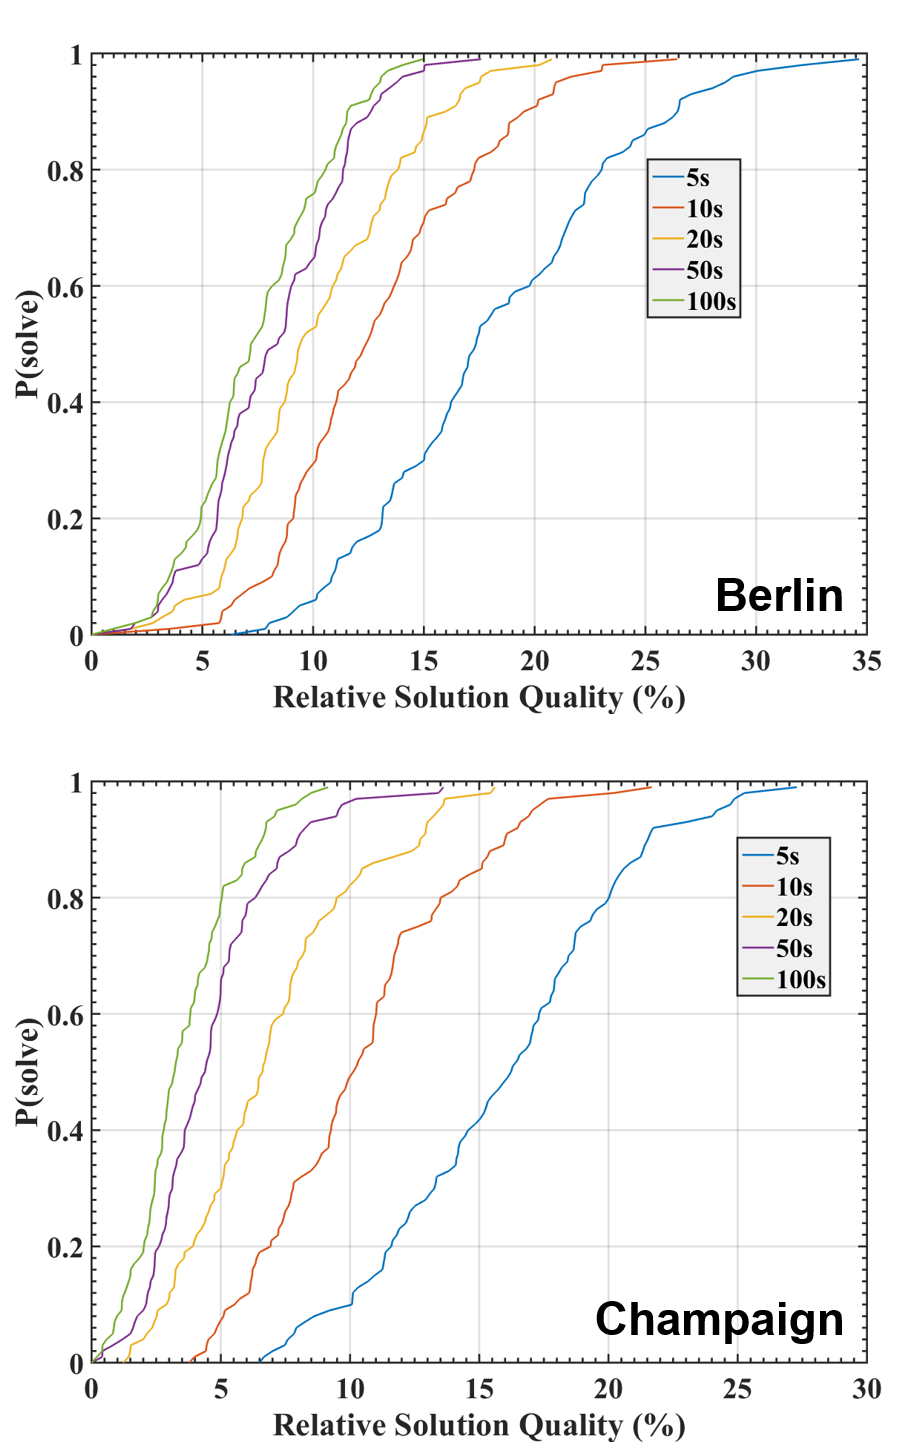
\includegraphics[width=0.35\textwidth]{F3-GA-SQD}
%     \caption{SQD plot using GA for Berlin and Champaign}
%     \label{fig: GA-SQD}
% \end{figure}

% \begin{figure}[h]
%     \centering
%     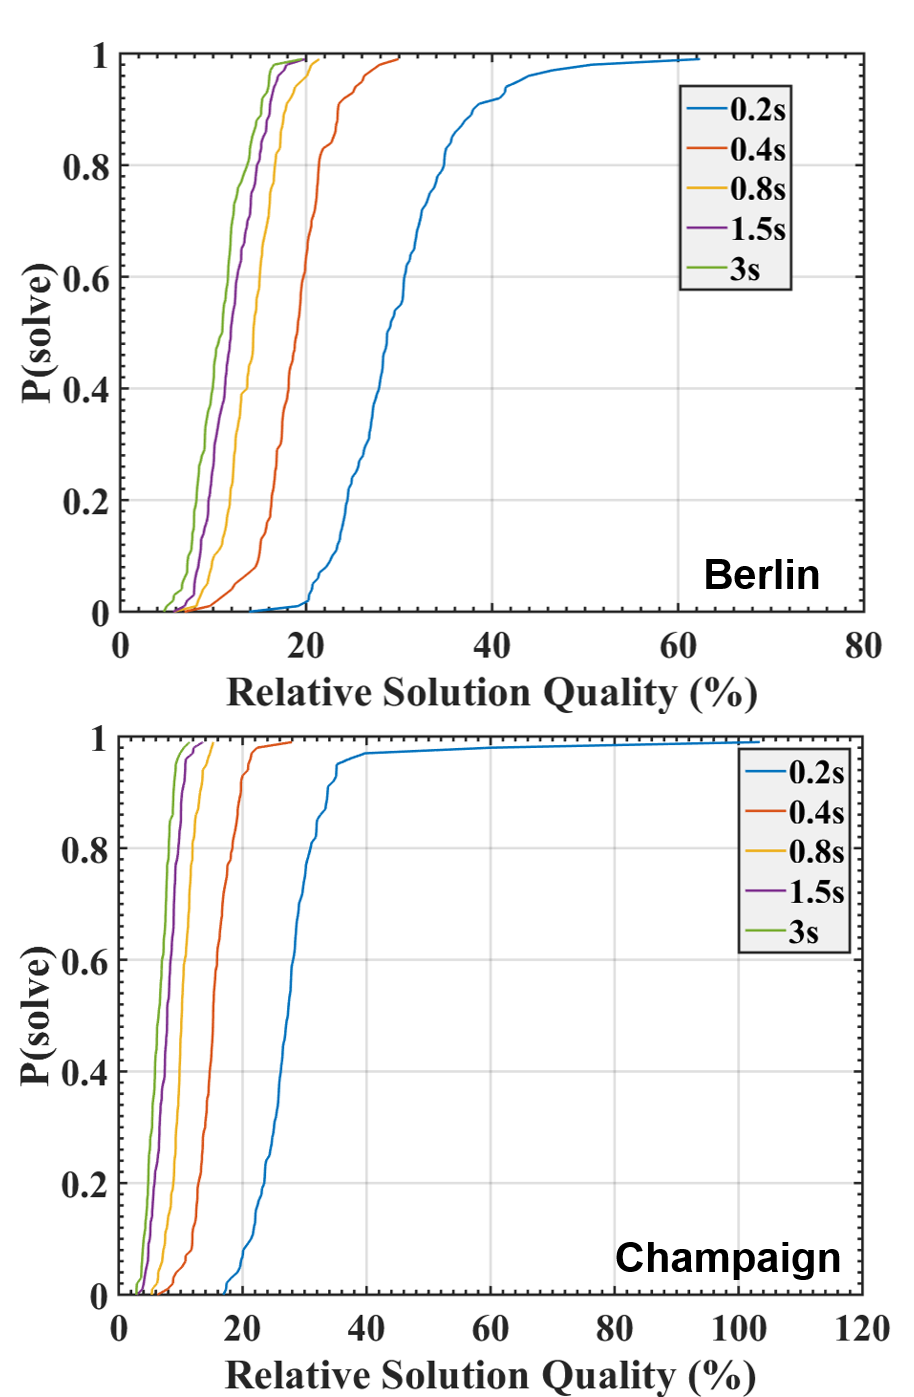
\includegraphics[width=0.35\textwidth]{F4-SA-SQD}
%     \caption{SQD plot using SA for Berlin and Champaign}
%     \label{fig: SA-SQD}
% \end{figure}
\begin{figure}
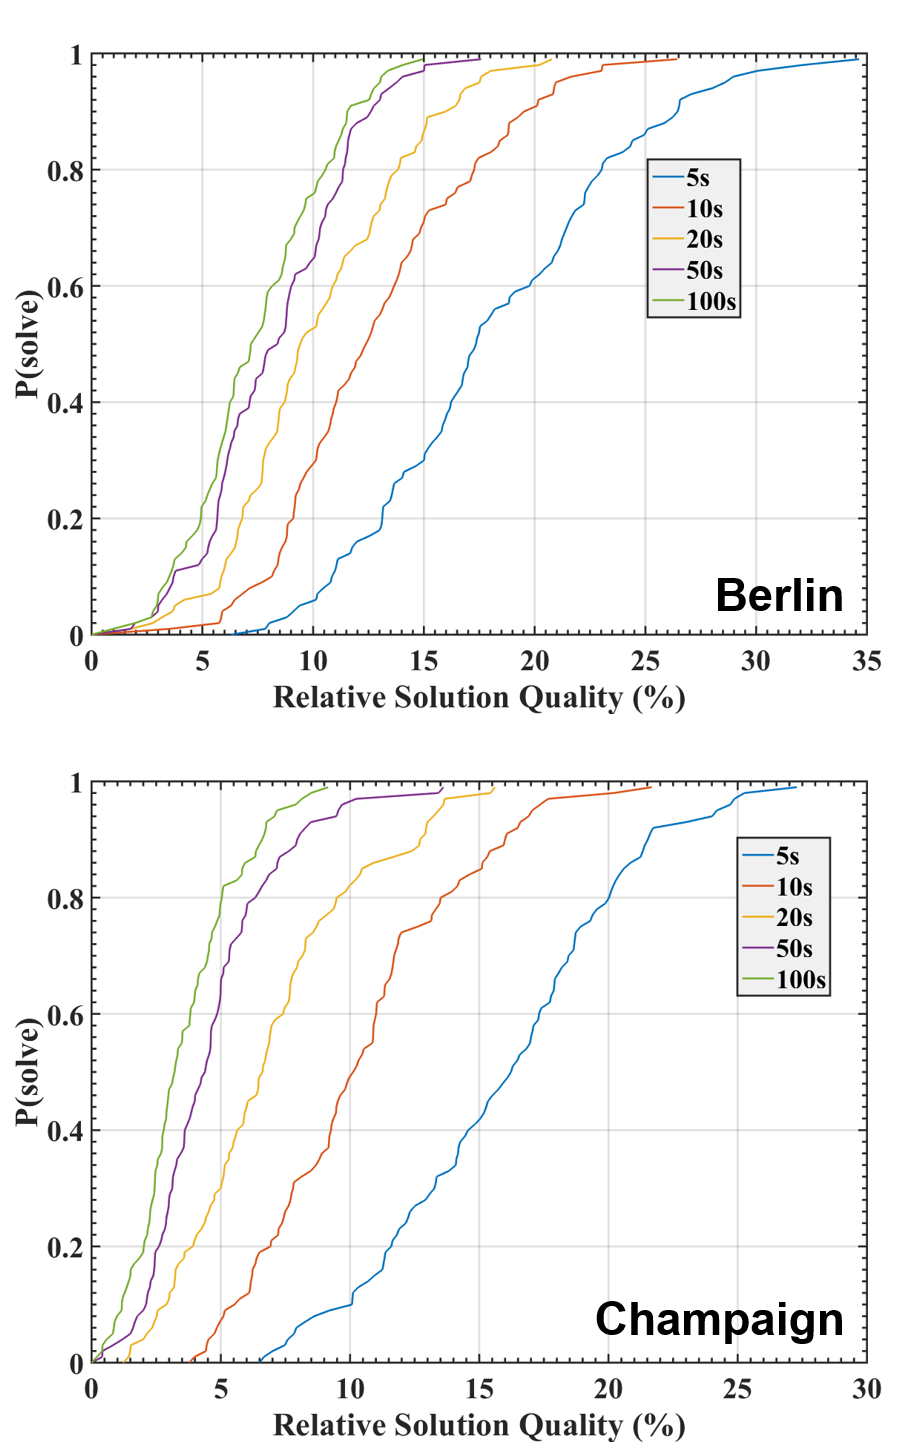
\includegraphics[width=2.5in]{F3-GA-SQD}
\caption{SQD plot using GA for Berlin and Champaign}
\label{fig: GA-SQD}
\end{figure}

\begin{figure}
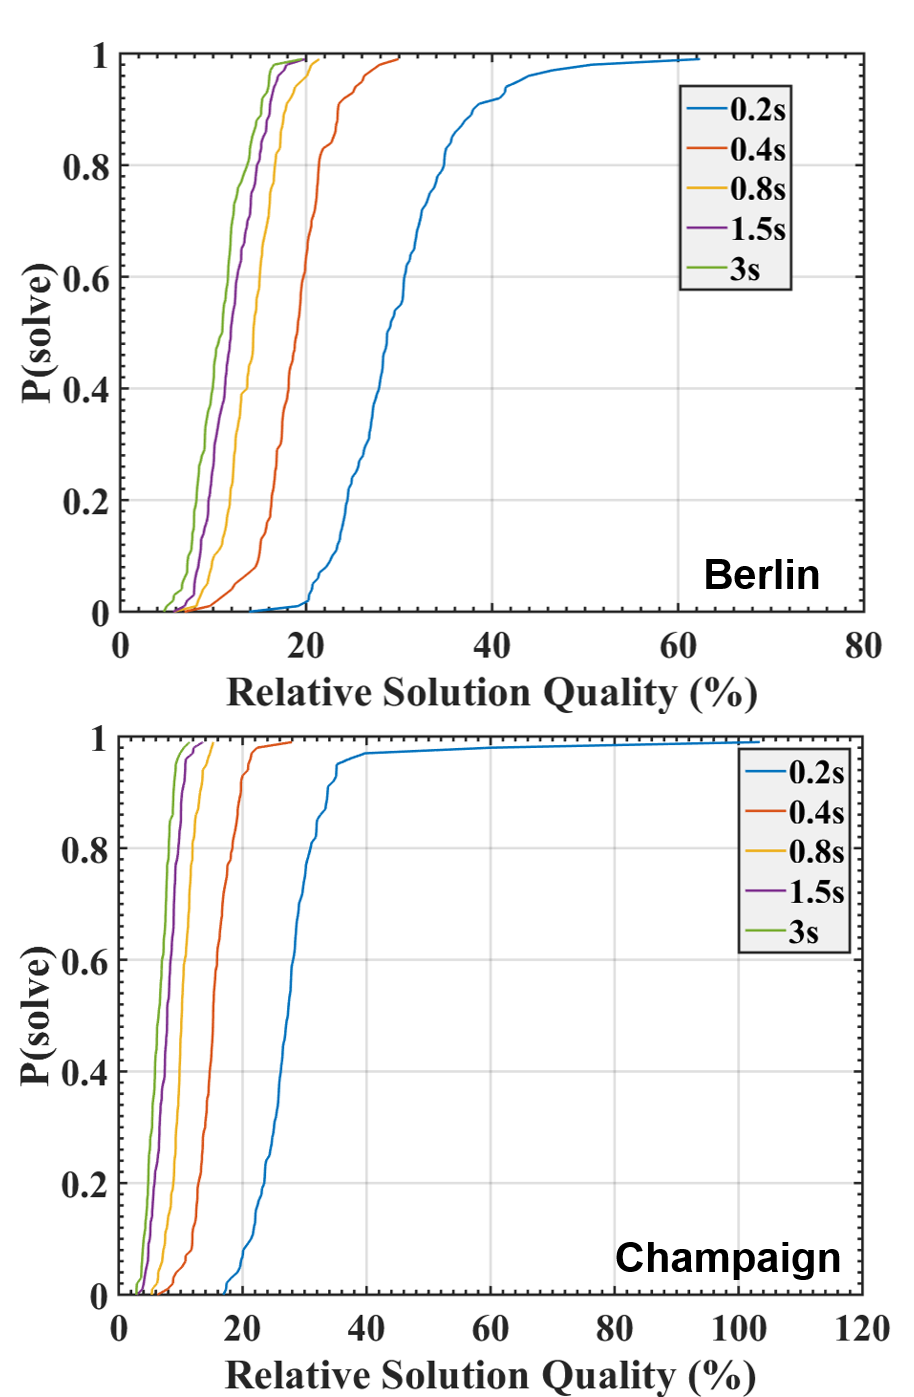
\includegraphics[width=2.5in]{F4-SA-SQD}
\caption{SQD plot using SA for Berlin and Champaign}
\label{fig: SA-SQD}
\end{figure}




\subsubsection{Box plots}
\hfill\\
The box plots for running times are shown in Figure \ref{fig: Box}. Note that this figure shows the minimum runtimes needed for solutions better than $(1+20\%) OPT$. For each case, the box plot includes maximum, minimum results, median and quartiles (25\% and 75\%). 99\% and 1\% values are also represented by the crosses, and mean value is represented by the square.\\
\hfill\\
From the box plots, there are only a few large outlier data points (<3) based on the results from 100 independent numerical experiments. Therefore, the performance of these two algorithms are stable and robust. The box plots also show that the running time is varying due to random seeds. We can see that SA can quickly converge to a satisfying solution and take less time than GA. 

\begin{figure}
\centering
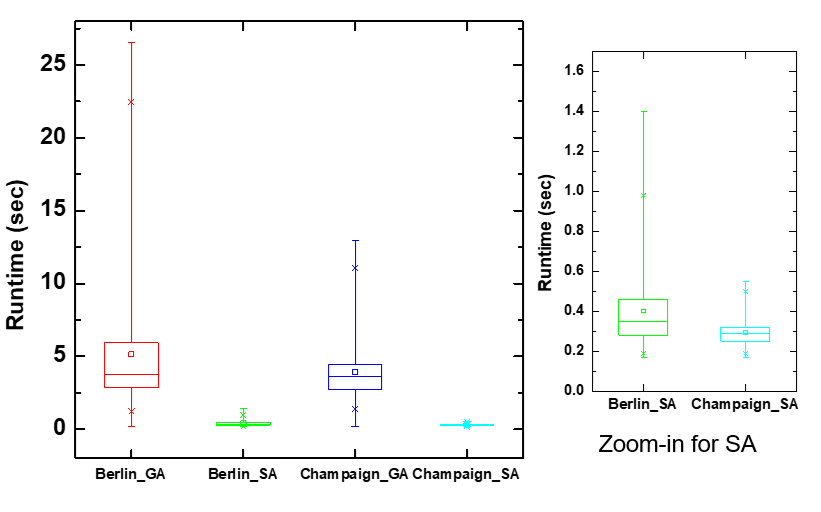
\includegraphics[width=3.5in]{F5-BoxPlot}
\caption{Box plot using GA and SA for Berlin and Champaign (right plot: zoom-in for SA)}
\label{fig: Box}
\end{figure}

\section{Discussion}
\subsection{Branch and Bound algorithm}
\hfill\\
A branch-and-bound algorithm consists of a systematic enumeration of all candidate solutions, where large subsets of fruitless candidates are discarded by using upper and lower estimated bounds of the quantity being optimized. For the implementation of Branch-and-Bound algorithm, we’ve considered various strategies, including random selection, assignment-problem strategy, and penalty-based selection. Since penalty-based selection will select the smallest extra costs for the current reduced matrix, thus will obtain a possibly lowest lower bound for the current step, we choose this strategy to search through the branches. In principle, BnB algorithm can obtain the exact optimal solution given enough time. However, since the worst case time complexity remains the same as that of the Brute Force, which is $O(2^n)$, it may take extremely long time. As we observed in the results, the cities with large input size (>55) cannot be solved within two days, and we can only obtain solutions as good as ~$(1+30\%)$OPT within 48h runtime.
\subsection{Approximation algorithm}
\hfill\\
MST-Approximation algorithm takes $O(n^2)$ and is the fastest one among the four algorithms. However, although it can guarantee an approximation ratio of 2, its errors are often larger than those of optimized local search algorithms as tested.

\subsection{Genetic Algorithm}
\hfill\\
Genetic algorithm has more capability to find the overall optimal solution. We found that the number of chromosomes in the population, crossover probability and mutation probability play important roles to improve the accuracy and efficiency of the algorithm. Based on many tries, we set the number of chromosomes in the population as 20 if the number of nodes in the city is more than 90. And the probability of mutation is set as 0.1. Otherwise, the number of chromosomes is set as 40 and the probability of mutation is set as 0.01. The probability of crossover is set as 0.8 regardless of the number of nodes in the city.

\subsection{Simulated Annealing algorithm}
\hfill\\
Simulated annealing algorithm is easy to implement. However, based on the implementation, SA algorithm gets stuck to local minimum easily. In addition, the quality of the output strongly depends on the initial value. 
In our implementation, we normalized the probability of taking new solution over the old one in the Metropolis condition as following:
\[P(s', s)=\Big\{
\begin{tabular}{cc}
1 & if \(f(s') < f(s)\)\\
\(exp \left\{
\frac{f(s)-f(s')}{Tf(s)}
\right\}
\) & otherwise
\end{tabular}
\]
where \(f(s)\) and \(f(s')\) is the total length of new solution and old solution respectively.\\
The temperature is updated using exponential relation shown below:
\[T=Te^{-kt_c}\]
Where \(t_c\) is the cutoff time. We would like the temperature to drop to 20\% of the initial temperature. Thus, the constant \(k\) can be derived as:
\[k=\frac{3.912}{t_c}\]
With different cutoff time, the speed of temperature decrease is also different, which would probability improve the output quality.


\section{Conclusions}
In this project, we have implemented four different algorithms to solve the NP-complete problem – Traveling Salesperson Problem (TSP). For the exact solutions, we used penalty-based selection strategy in the Branch-and-Bound algorithm to obtain good quality of lower bound. Over half of all the given cases have been solved within 1.5 hours. Then we implemented MST-approximation, which is a classical algorithm to solve NP-complete problem within short time frame. For all the given cases, it takes less than 0.1 sec to run the algorithm, and can achieve solution qualities better than 40\%. \\ 
\hfil\\
We have also implemented two local search algorithms: generic algorithm (GA) and simulated annealing algorithm (SA). Local search algorithms are generally fast and can produce satisfactory results with carefully optimized parameters. All the given cases can be solved with qualities better than 15\% within 2 minutes in our experiments.   

\begin{acks}
D. Han and S. Xiong conducted the algorithm design, implementation and analysis for the BnB and Approximation algorithms. C. Ye and Y. Zhou conducted the algorithm design, implementation and analysis for the local search algorithms. All of the authors contributed to the manuscript with the  sections corresponding to each algorithm. \\
\hfill\\
We would like to thank the NOES solver to offer Concorde to solve symmetric TSP at https://neos-server.org/neos/solvers/co:concorde/ -TSP.html.

\end{acks}

% \bibliographystyle{ACM-Reference-Format}
\bibliographystyle{unsrtnat}
\bibliography{CSE6140-T31}


\end{document}
